\documentclass[12pt, letterpaper]{article}
\usepackage{graphicx} % needed for images
\usepackage[export]{adjustbox} % needed for adjustable images
\usepackage{flafter} % needed for figures
\usepackage{hyperref} % needed for a clickable table of contents
% \usepackage{cleveref}
\usepackage{subfiles} % needed for a subfile structure
\usepackage[table]{xcolor}
\usepackage{fancyhdr} % needed for fancy header 
\usepackage{listings}
\usepackage{tabularx}
\usepackage{array}
\usepackage{color}
\usepackage{colortbl}
\usepackage{lineno}

\graphicspath{ {images/} }

\pagestyle{fancy}
\fancyhf{}
\fancyhead[LE,RO]{REST API - Distributed Computing}
\fancyfoot[LE,RO]{\thepage}
\renewcommand{\headrulewidth}{1pt}
\renewcommand{\footrulewidth}{1pt}

% information
\title{%
    \begin{center}
	
\includegraphics[width=4cm,height=3cm]{udl.png}
    \end{center}
    \line(1,0){250}\\[0.3cm]
    \textbf{Cloud Service}
    \line(1,0){250}
    \\[0.5cm]
	\large Rest API - Grau en Enginyeria Informàtica
}
\author{Artur Cullerés Cervera \\ Roger Fontova Torres}
\date{\today}

% document
\begin{document}
    
% title
\maketitle
\thispagestyle{empty}
\newpage
\tableofcontents
\listoffigures
% \listoftables
\newpage
\
\newpage

% begin contents

\section{Introduction}
\label{sections:introduction}
In this project, we have been assigned the task to create a REST API that stores Users, Homes and Sensors with its relations into a Relational Database. We decided to work with Spring Boot since it has a very accessible learning curve. Also, we decided to use the ApiFirst principle, which is about defining first the API and then implementing it according to its definition instead of implementing at the same time it is defined. \\

We have approached this project as if it was for an application for an IoT network where you can have a user account, with your homes and sensors. This means that operations to entities that don't belong to you, are forbidden.



\section{OpenApi 3.0}
In order to apply this principle, we used OpenApi 3.0, which is a specification to describe, produce and consume RESTful web services. Also, it exists a code generator that generates all the code (only the structure) the clients will interact directly with (it creates the structure of the endpoints and the DTOs). Since we use Spring Boot, we decided to use the spring generator. \\

Thanks to the specification, we have an accessible documentation to know how to call each endpoint, what does it return, etc.

\section{Architecture}
We decided to use the MVC architecture since it is the most used in REST APIs. We also used a mapping system between DTOs and DAOs, since we might not want to show all the columns that we have in the database. In order to do that, we have used the mapstruct library, which enables us to easyly create mappers.

\begin{figure}[!htbp]
    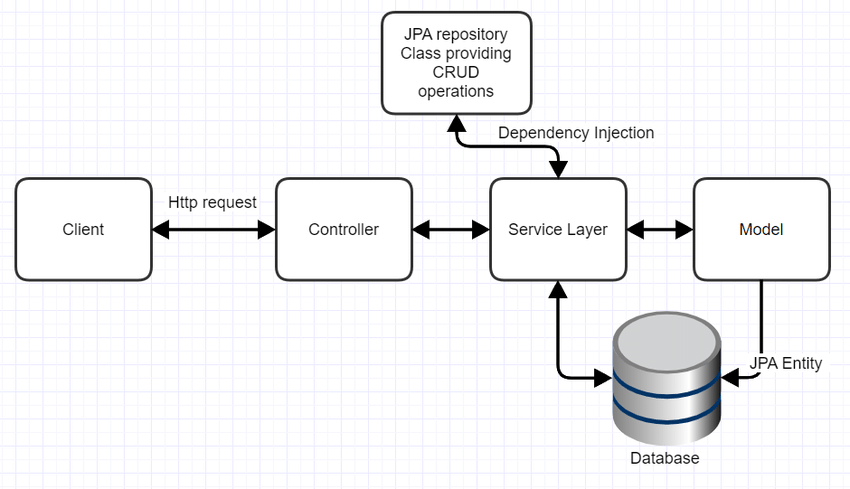
\includegraphics[scale=0.5]{mvc.png}
    \centering
    \caption{MVC architecture}
    \label{mvc}
\end{figure}

\newpage




\section{Login system}
In order to implement a login system, we used the JWT library. This library is very customizable and helps with the control of "exposing" the endpoints. When the authorization endpoint is called, and the credentials are correct, it generates and return a token, which will be used to validate our identity each time we want to call any endpoint. \\

The only endpoints that are available without being logged are the authentication endpoint and the sing-up endpoint.

\section{Conclusions}
With this project we have basically learnt how a RESTful API works. This includes the naming of the every component (endpoints, DAO, DTO, controllers, etc), how to define an API in a correct way, how to use mappers, how do tokens work and their utilities, just to name some. \\

Finally, we will leave the link to the \href{https://github.com/RogerFontovaTorres/iot-rest}{github repository} of the project so anyone can access the source code. \\

In order to see the API specification, you must copy the code form the file swagger.yaml, inside the folder resources, to this \href{https://editor.swagger.io/}{editor}.


\end{document}
